\newpage
\section{Evaluation}
\label{sec:eval}
In this section, we present our evaluation study of \tool. The results
are presented in three parts, where we first present the distribution of
weak consistency requirements on benchmark programs. Second, we presents
our studies on the performance of programs running on various
consistency levels and finally, we present the complexity and
perforamnce results from our study of implementing 
a well-understood 
ad-hoc prevention mechanism for lost-updates anomaly, compared to writing
the same program in \tool. 
%
%
% 
\subsection{Weak Consistency in Benchmark Programs}
\begin{figure}[b]
\centering
\begin{center}
\begin{scriptsize}
\begin{tabular}{|l |  l | l|} 
\hline
 \multicolumn{1}{|c}  {\bf Benchmark} & \multicolumn{1}{c} {\bf
 Consistency} & \multicolumn{1}{c|}  {\bf
 Description}\\ [0.5ex] 
\hline
Counter  & MR & {Monotonicly increasing counter, e.g.
YouTubes' watch 
count}\\ \hline
DynamoDB  & RMW & {Integer register allowing various conditional puts and gets} \\ \hline
Online Store & RMW &  {Online store with shopping carts
and modifiable item prices} \\ \hline
Bankaccount  & 2VIS $\wedge$ RMW & {Offering deposit, withdraw and get balance operations}\\ \hline
Shopping List   &  MW $\wedge$ RMW & {A shopping list with
concurrent adds and deletes functionality}\\ \hline 
Microblog  &  MW, RMW & {A Twitter-like application modeled after
Twissandra}\\\hline
Rubis  & RMW, RMW$\wedge$2VIS & {eBay-like
application with browsing, supporting user wallet} \\
\hline
\end{tabular}
\end{scriptsize}
\end{center}
\caption{Fine-grained consistency requirement in benchmark programs}
\label{fig:dist_table}
\end{figure}

In this section, we present seven different benchmark applications we collected,
in which various types of anomalous behavior under eventual consistency have been
detected. We present these programs and their detected consistency
requirements, in figure \ref{fig:dist_table}. 
For example, two following anomalies have been detected for operations
of the microblog application:
\begin{enumerate}
  \item When Alice unfollows Donald, but later
  sees more tweets from him. This is because the
  $\mathtt{getFolloweeList}$ operation did not witness the effect of the
  $\mathtt{unfollow}$
  operation; a clear example of lost-updates anomaly which can be
  prevented by RMW guarantee.
  \item When Donald posts a series of tweets, but after Alice refreshes
  her timline, only sees the fifth tweet. This can be prevented by
  requiring $\mathtt{getTweet}$ operation to return only tweets, whose prior
  tweets are also visible; which is exacly what is provided by
  enforcing MW contract.
\end{enumerate}

In addition to having a large number of operations each of which might
require a different level of consistency, above examples also show how
in practice, some programs might inlcude
operations that are involved in \emph{multiple} types of anomalies. For example
the $\mathtt{getBalance}$ operation of the bank account application above,
shows two different types of anomalies, whose prevention requires 2VIS
\emph{and} RMW. The possiblity of showing \emph{combinations} of
anomalies, considering the large number of known anomalies, shows the
inefficiency of any consistency enforcement technique specific to a
certain type of anomaly.
%
%
%
\subsection{Latency and Staleness Comparison}
\begin{figure}[t]
        \centering
	\begin{subfigure}[t]{0.25\textwidth}
	\centering
	\hspace{-13mm}
	
\includegraphics[scale=0.22]{Figures/latency.pdf}
	\subcaption*{ \hspace{-10mm} (a) Latency}
	\end{subfigure}
	\begin{subfigure}[t]{0.36\textwidth}
	\centering
	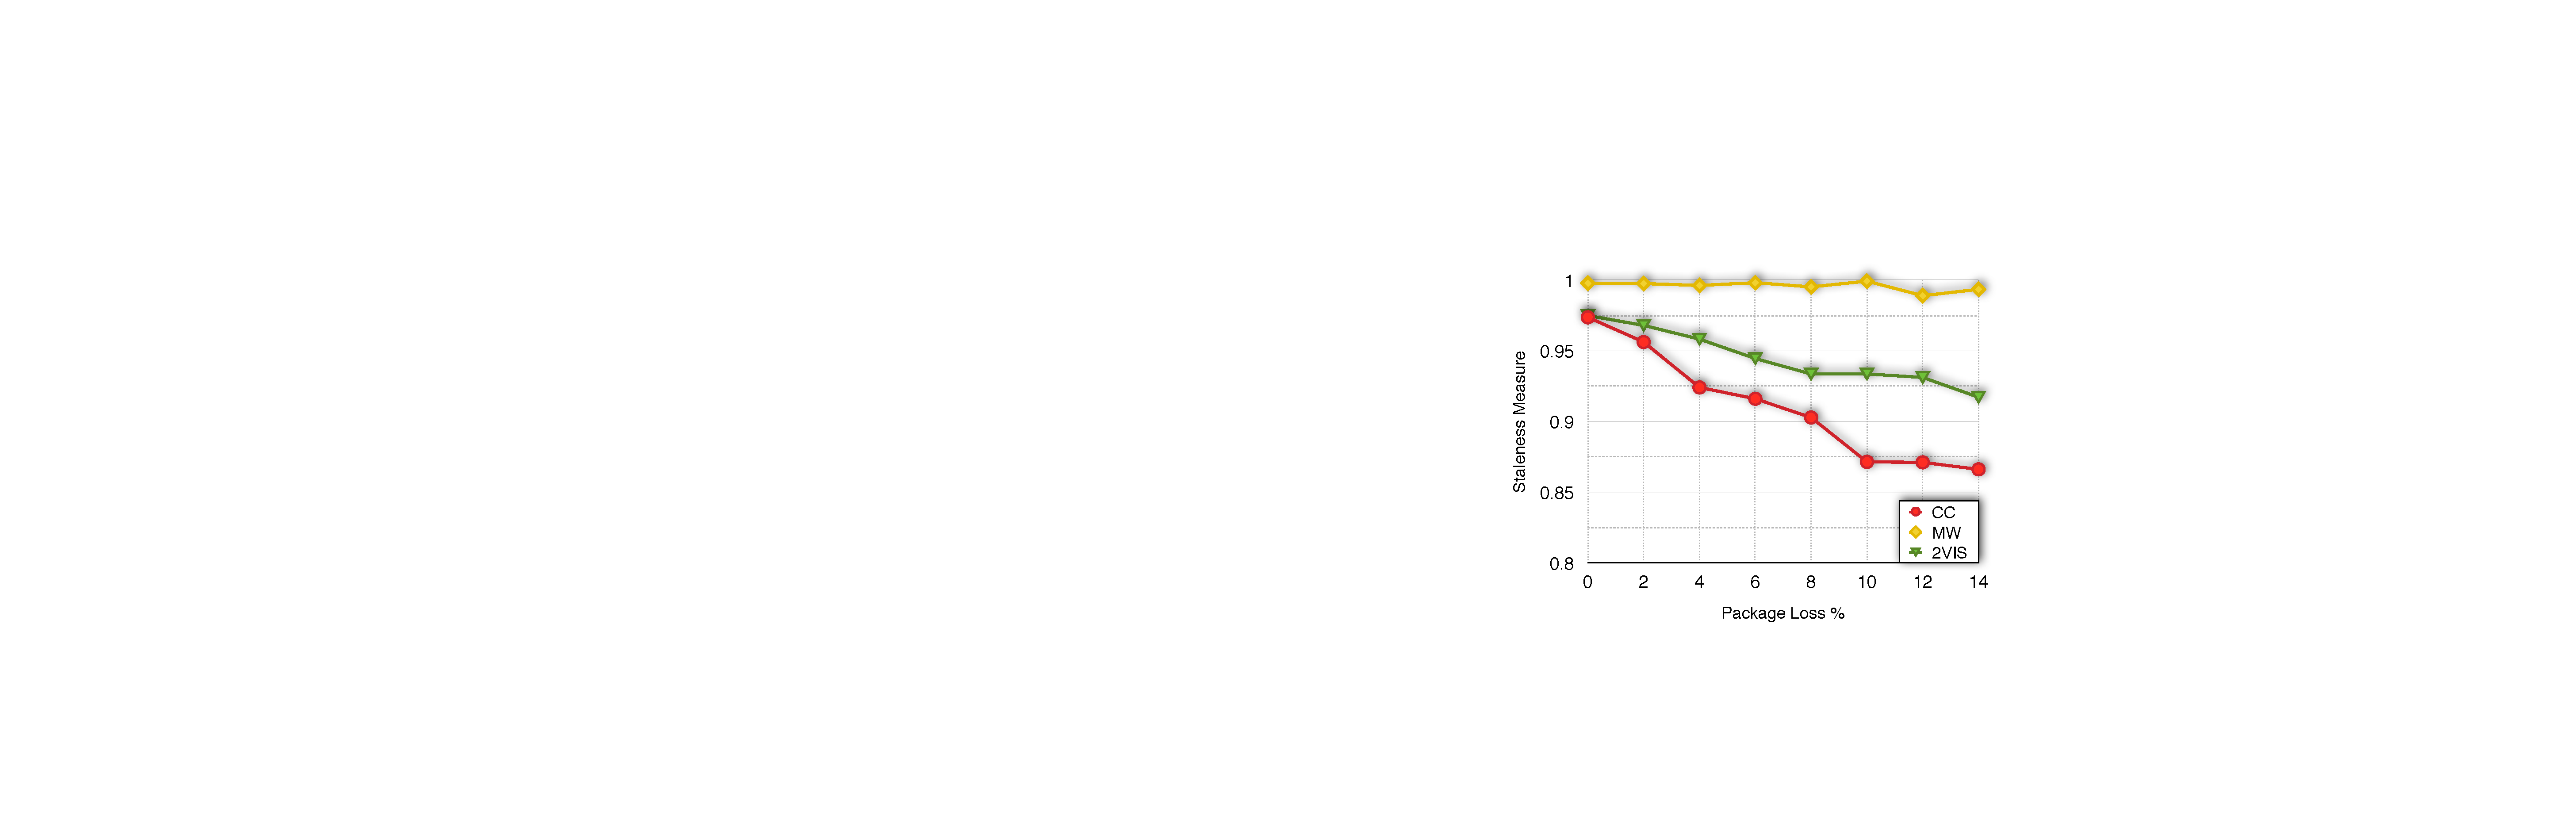
\includegraphics[scale=0.22]{Figures/staleness.pdf}
	\subcaption*{ \hspace{-1mm} (b) Staleness}
	\label{subfig:comment_example}
	\end{subfigure} 
	\begin{subfigure}[t]{0.28\textwidth}
	\centering
	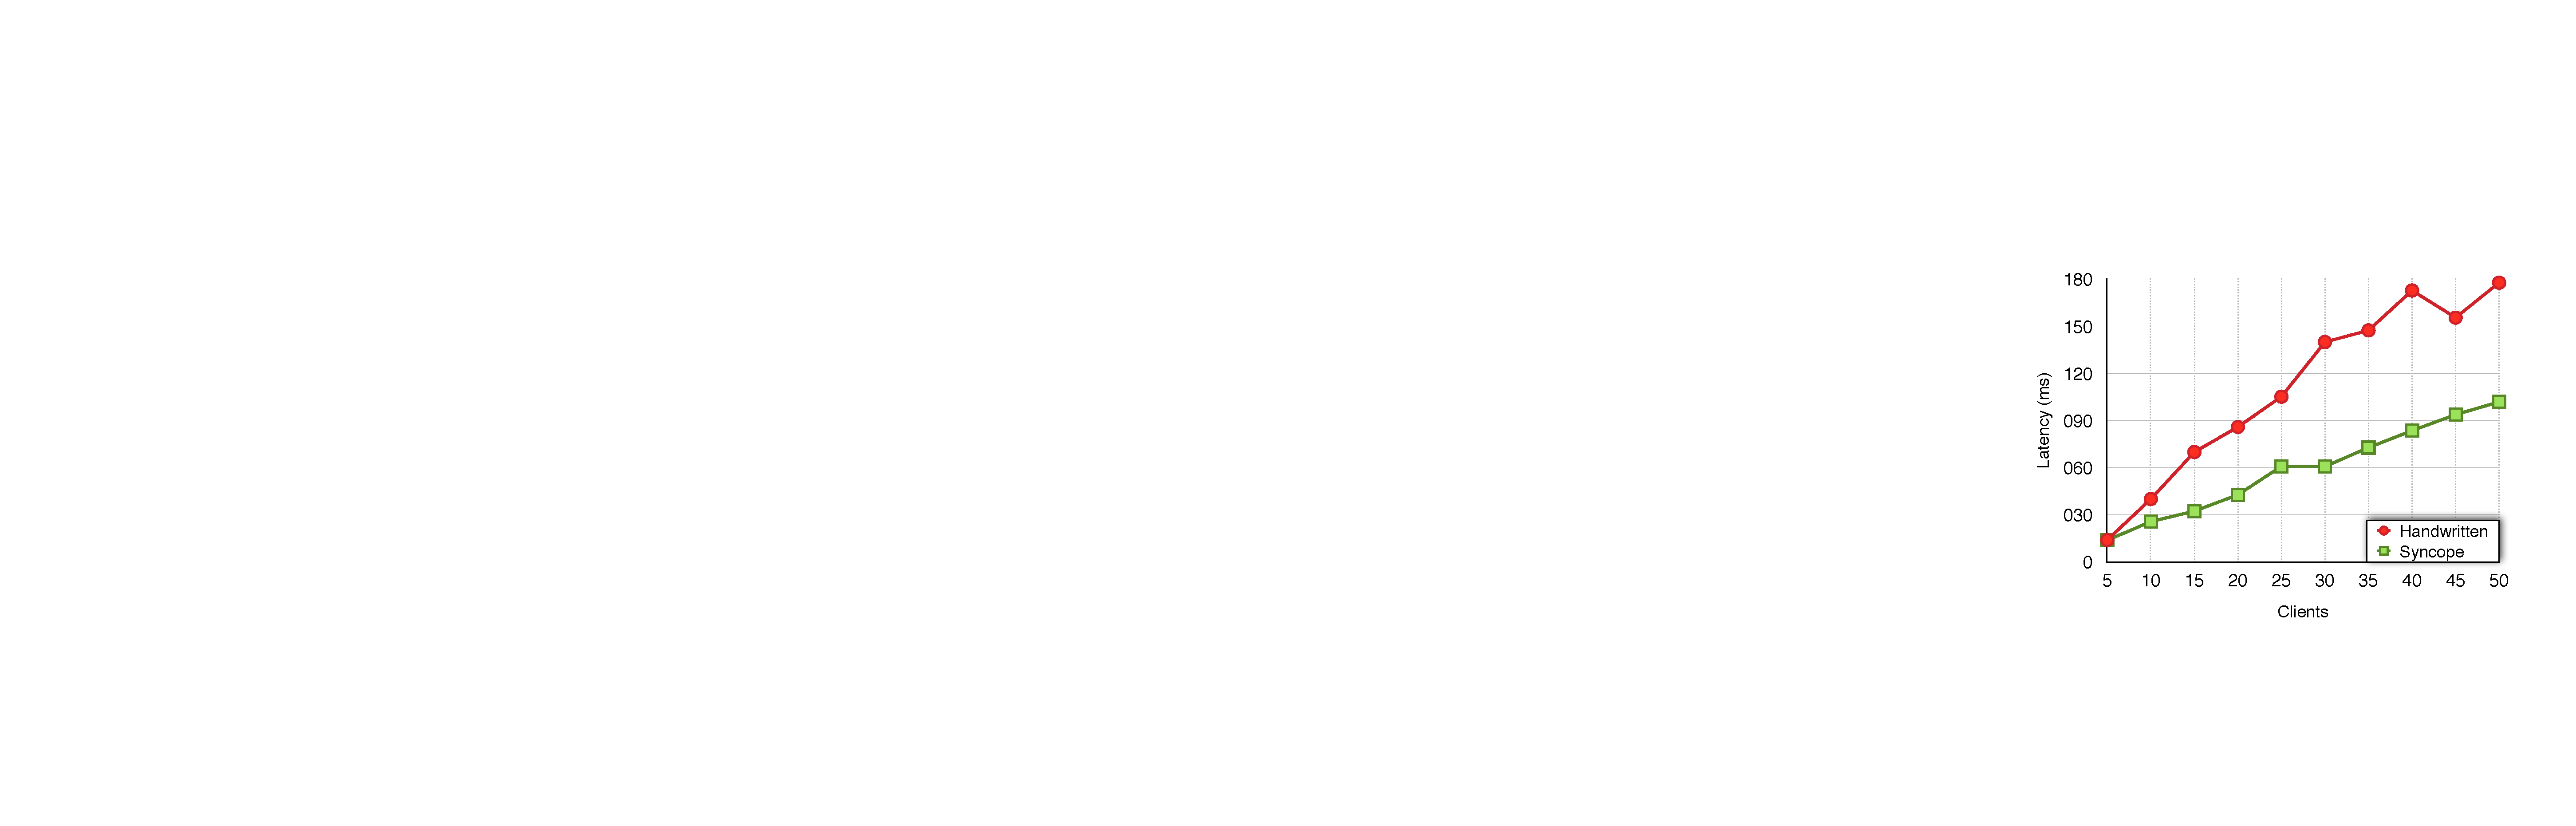
\includegraphics[scale=0.22]{Figures/comparison.pdf}
	\subcaption*{ \hspace{8mm} (c) Manual RMW}
	\label{subfig:comment_example}
	\end{subfigure} 
\\ \hrulefill
\caption{A distributed application for comment section
management}
\label{fig:eval}
\end{figure}





















\newpage
\subsection{Ad-hoc vs \tool }
\newpage
